\subsection{Compiling and installing the kernel}

\begin{frame}[fragile]
  \frametitle{Kernel compilation}
  \begin{columns}
  \column{0.7\textwidth}
  \code{make}
  \begin{itemize}
    \item Only works from the top kernel source directory
    \item Should not be performed as a privileged user
    \item Run several {\bf j}obs in parallel. Our advice: \code{$(nproc)} to
      fully load the CPU and I/Os at all times.\\
          Example: \code{make -j20}
    \item To {\bf re}compile faster (7x according to some benchmarks),\\
	  use the \code{ccache} compiler cache:\\
          \code{export CROSS_COMPILE="ccache arm-linux-"}
  \end{itemize}
  \column{0.3\textwidth}
    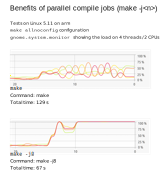
\includegraphics[width=\textwidth]{slides/linux-kernel-intro-building/parallel-make-benefits.pdf}
  \end{columns}
\end{frame}

\begin{frame}
  \frametitle{Kernel compilation results}
  \begin{itemize}
    \item \code{arch/<arch>/boot/Image}, uncompressed kernel image that
      can be booted
    \item \code{arch/<arch>/boot/*Image*}, compressed kernel images that
      can also be booted
      \begin{itemize}
      \item \code{bzImage} for x86, \code{zImage} for ARM,
      \code{Image.gz} for RISC-V, \code{vmlinux.bin.gz} for ARC, etc.
      \end{itemize}
    \item \code{arch/<arch>/boot/dts/<vendor>/*.dtb}, compiled Device Tree Blobs
    \item All kernel modules, spread over the kernel source tree, as
      \code{.ko} ({\em Kernel Object}) files.
    \item \code{vmlinux}, a raw uncompressed kernel image in the ELF
      format, useful for debugging purposes but generally not used for
      booting purposes
  \end{itemize}
\end{frame}

\begin{frame}
  \frametitle{Kernel installation: native case}
  \begin{itemize}
  \item \code{sudo make install}
    \begin{itemize}
    \item Does the installation for the host system by default
    \end{itemize}
  \item Installs
    \begin{itemize}
    \item \code{/boot/vmlinuz-<version>} \\
      Compressed kernel image. Same as the one in
      \code{arch/<arch>/boot}
    \item \code{/boot/System.map-<version>}\\
      Stores kernel symbol addresses for debugging purposes
      (obsolete: such information is usually stored in the kernel itself)
    \item \code{/boot/config-<version>}\\
      Kernel configuration for this version
    \end{itemize}
  \item In GNU/Linux distributions, typically re-runs the bootloader configuration
    utility to make the new kernel available at the next boot.
  \end{itemize}
\end{frame}

\begin{frame}
  \frametitle{Kernel installation: embedded case}
  \begin{itemize}
  \item \code{make install} is rarely used in embedded development, as the
    kernel image is a single file, easy to handle.
  \item Another reason is that there is no standard way to deploy and
    use the kernel image.
  \item Therefore making the kernel image available to the target is
    usually manual or done through scripts in build systems.
  \item It is however possible to customize the \code{make install}
    behavior in \code{arch/<arch>/boot/install.sh}
  \end{itemize}
\end{frame}

\begin{frame}
  \frametitle{Module installation: native case}
  \begin{itemize}
  \item \code{sudo make modules_install}
    \begin{itemize}
    \item Does the installation for the host system by default, so
      needs to be run as root
    \end{itemize}
  \item Installs all modules in \code{/lib/modules/<version>/}
    \begin{itemize}
    \item \code{kernel/}\\
      Module \code{.ko} (Kernel Object) files, in the same directory
      structure as in the sources.
    \item \code{modules.alias}, \code{modules.alias.bin}\\
      Aliases for module loading utilities
    \item \code{modules.dep}, \code{modules.dep.bin}\\
        Module dependencies. Kernel modules can depend on other modules,
        based on the symbols (functions and data structures) they use.
    \item \code{modules.symbols}, \code{modules.symbols.bin}\\
      Tells which module a given symbol belongs to (related to
      module dependencies).
    \item \code{modules.builtin}\\
      List of built-in modules of the kernel.
    \end{itemize}
  \end{itemize}
\end{frame}

\begin{frame}
  \frametitle{Module installation: embedded case}
  \begin{itemize}
  \item In embedded development, you can't directly use
    \code{make modules_install} as it would install target modules
    in \code{/lib/modules} on the host!
  \item The \code{INSTALL_MOD_PATH} variable is needed to generate
    the module related files and install the modules in the target
    root filesystem instead of your host root filesystem (no need
    to be root):\\
    \code{make INSTALL_MOD_PATH=<dir>/ modules_install}
  \end{itemize}
\end{frame}

\begin{frame}[fragile]
  \frametitle{Kernel cleanup targets}
  \begin{columns}
    \column{0.8\textwidth}
    \small
    \begin{itemize}
    \item From \code{make help}:
    \begin{block}{}
    \begin{minted}[fontsize=\scriptsize]{console}
Cleaning targets:
  clean           - Remove most generated files but keep the config and
                    enough build support to build external modules
  mrproper        - Remove all generated files + config + various backup files
  distclean       - mrproper + remove editor backup and patch files
     \end{minted}
     \end{block}
    \item If you are in a git tree, remove all files not tracked (and
      ignored) by git:\\
      \code{git clean -fdx}
    \end{itemize}
    \column{0.2\textwidth}
    
\includegraphics[width=0.9\textwidth]{slides/linux-kernel-intro-building/kernel-mrproper.png}
  \end{columns}
\end{frame}

\begin{frame}
  \frametitle{Kernel building overview}
  \begin{center}
    \includegraphics[height=0.8\textheight]{slides/linux-kernel-intro-building/kernel-building-overview.pdf}
  \end{center}
\end{frame}
